
%(BEGIN_QUESTION)
% Copyright 2008, Tony R. Kuphaldt, released under the Creative Commons Attribution License (v 1.0)
% This means you may do almost anything with this work of mine, so long as you give me proper credit

%Sketch a circuit whereby this loop-powered pressure transmitter sends a signal to an analog current meter (acting as a remote pressure gauge).  Include any necessary power sources in your completed circuit:

Tegn en krets der trykktransmitteren sender et signal til ampermeteret (som brukes for å indikere trykk i et kontrollrom). Ta med nødvendig strømforsyning. 

\vskip 50pt

$$\includegraphics[width=15.5cm]{i02670x01.eps}$$

\vfil 

\underbar{file i02670no}
\eject
%(END_QUESTION)





%(BEGIN_ANSWER)

This is a graded question -- no answers or hints given!

%(END_ANSWER)





%(BEGIN_NOTES)

A vital principle to bear in mind with any 4-20 mA loop-powered transmitter circuit is that a loop-powered instrument acts as a {\it load} and not a {\it source}, even though it is the component regulating current.  Thus, a loop-powered transmitter drops voltage in the same manner that a resistor drops voltage (i.e. + on the side where conventional-flow current enters, - on the side where conventional-flow current exits).

\vskip 10pt

This is just one possible solution:

$$\includegraphics[width=15.5cm]{i02670x02.eps}$$

\vskip 10pt

Here is an alternative solution:

$$\includegraphics[width=15.5cm]{i02670x03.eps}$$

\filbreak

A good problem-solving technique to apply here is sketching arrows showing where conventional flow (current) enters and exits each component, based on its voltage polarity and its identity as either a source or a load.  Once these arrows are sketched, it becomes a trivial matter to connect tip-to-tail to form a series circuit:

$$\includegraphics[width=15.5cm]{i02670x04.eps}$$

{\it Any} connections that put the tip of one arrow connecting the tail of another will form a valid series circuit!


%INDEX% Pictorial circuit review (4-20 mA loop)

%(END_NOTES)


